\chapter{半导体中的电子}

\section{半导体的晶格结构与结合性质}

\subsection{金刚石型结构和共价键}

\ce{Si},\ce{Ge}等元素属于IV族元素,外层具有四个价电子。这些元素通过\textbf{共价键}结合形成晶体,晶格结构与\ce{C}元素的金刚石晶体的晶格相同,属于\textbf{金刚石型结构}。这种结构中,每个原子周围有四个近邻原子,组成正四面体结构。这四个原子处于正四面体的顶角上,它们与中心原子各自贡献一个价电子为两个原子共有,并形成共价键。金刚石结构的配位数是$4$。

\begin{figure}[H]
    \centering
\tikzset{every picture/.style={line width=0.75pt}} %set default line width to 0.75pt        

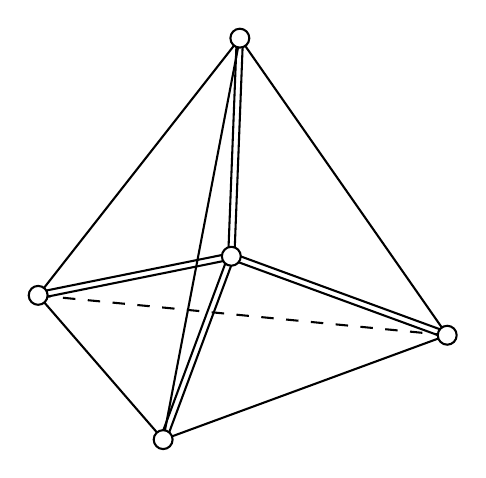
\begin{tikzpicture}[x=0.75pt,y=0.75pt,yscale=-1,xscale=1]
%uncomment if require: \path (0,333); %set diagram left start at 0, and has height of 333

%Flowchart: Extract [id:dp2941884800038894] 
\draw   (279.75,67.58) -- (242.81,261) -- (182.58,191.5) -- cycle ;
%Straight Lines [id:da11678715957846952] 
\draw    (279.75,67.59) -- (379.67,210.72) ;
%Straight Lines [id:da6291753538375728] 
\draw    (242.81,261) -- (379.67,210.72) ;
%Straight Lines [id:da792032373772936] 
\draw  [dash pattern={on 4.5pt off 4.5pt}]  (182.58,191.49) -- (379.67,210.72) ;
%Straight Lines [id:da16681599054483343] 
\draw [color={rgb, 255:red, 0; green, 0; blue, 0 }  ,draw opacity=1 ][fill={rgb, 255:red, 0; green, 0; blue, 0 }  ,fill opacity=1 ]   (281.25,67.64) -- (277.14,172.73)(278.25,67.53) -- (274.14,172.61) ;
%Straight Lines [id:da8617596562201413] 
\draw    (275.94,174.14) -- (182.88,192.96)(275.35,171.2) -- (182.28,190.02) ;
%Straight Lines [id:da5282358800451186] 
\draw    (276.16,171.26) -- (380.18,209.31)(275.13,174.08) -- (379.15,212.13) ;
%Straight Lines [id:da21390436106539057] 
\draw    (277.05,173.19) -- (244.21,261.52)(274.24,172.14) -- (241.4,260.48) ;
%Shape: Circle [id:dp8215196387479993] 
\draw  [fill={rgb, 255:red, 255; green, 255; blue, 255 }  ,fill opacity=1 ] (178.03,191.5) .. controls (178.03,188.98) and (180.07,186.94) .. (182.58,186.94) .. controls (185.1,186.94) and (187.14,188.98) .. (187.14,191.5) .. controls (187.14,194.01) and (185.1,196.05) .. (182.58,196.05) .. controls (180.07,196.05) and (178.03,194.01) .. (178.03,191.5) -- cycle ;
%Shape: Circle [id:dp656158588884858] 
\draw  [fill={rgb, 255:red, 255; green, 255; blue, 255 }  ,fill opacity=1 ] (275.2,67.59) .. controls (275.2,65.07) and (277.24,63.03) .. (279.75,63.03) .. controls (282.27,63.03) and (284.31,65.07) .. (284.31,67.59) .. controls (284.31,70.1) and (282.27,72.14) .. (279.75,72.14) .. controls (277.24,72.14) and (275.2,70.1) .. (275.2,67.59) -- cycle ;
%Shape: Circle [id:dp4448830323802311] 
\draw  [fill={rgb, 255:red, 255; green, 255; blue, 255 }  ,fill opacity=1 ] (375.11,210.72) .. controls (375.11,208.2) and (377.15,206.16) .. (379.67,206.16) .. controls (382.18,206.16) and (384.22,208.2) .. (384.22,210.72) .. controls (384.22,213.23) and (382.18,215.27) .. (379.67,215.27) .. controls (377.15,215.27) and (375.11,213.23) .. (375.11,210.72) -- cycle ;
%Shape: Circle [id:dp8703628065470996] 
\draw  [fill={rgb, 255:red, 255; green, 255; blue, 255 }  ,fill opacity=1 ] (271.09,172.67) .. controls (271.09,170.15) and (273.13,168.11) .. (275.64,168.11) .. controls (278.16,168.11) and (280.2,170.15) .. (280.2,172.67) .. controls (280.2,175.18) and (278.16,177.22) .. (275.64,177.22) .. controls (273.13,177.22) and (271.09,175.18) .. (271.09,172.67) -- cycle ;
%Shape: Circle [id:dp849985969268054] 
\draw  [fill={rgb, 255:red, 255; green, 255; blue, 255 }  ,fill opacity=1 ] (238.25,261) .. controls (238.25,258.48) and (240.29,256.44) .. (242.81,256.44) .. controls (245.32,256.44) and (247.36,258.48) .. (247.36,261) .. controls (247.36,263.52) and (245.32,265.56) .. (242.81,265.56) .. controls (240.29,265.56) and (238.25,263.52) .. (238.25,261) -- cycle ;
\end{tikzpicture}
    \caption{正四面体结构}
    \label{fig:tetrahedron}
\end{figure}

实验测得 \ce{Si}和 \ce{Ge}的晶格常数$a$分别为$0.543102\ \mathrm{nm}$和$0.565791\ \mathrm{nm}$。

\begin{figure}[H]
    \centering
    \includegraphics{diamond.png}
    \caption{金刚石晶胞}
    \label{fig:diamond}
\end{figure}

\subsection{闪锌矿型结构和混合键}

III族元素 \ce{Al}, \ce{Ga}, \ce{In}和V族元素 \ce{P}, \ce{As}, \ce{Sb}形成的III-V族化合物是半导体材料,它们具有闪锌矿型结构,这种结构和金刚石结构相似,但它由两种不同的原子组成。这种结构依靠共价键结合,但有一定的离子键成分。

\subsection{纤锌矿型结构}

纤锌矿型结构与闪锌矿型结构类似,以正四面体结构为基础构成,但它具有六方对称性。其结合性质也具有一定的离子性。

\section{半导体中的电子状态和能带}

\subsection{半导体中的电子状态和能带}

晶体中的电子介于孤立原子中的电子和自由电子之间。孤立原子中的电子在原子核和其他电子的势场中运动;自由电子在零势场中运动。

首先介绍自由电子的运动。

微观粒子具有波粒二象性。一个质量$m_0$的自由电子以速度$\bm v$运动,其动量与能量为:
\begin{align}
    &\bm p=m_0 \bm v\label{eq:free_momentum}\\
    &E=\frac{1}{2}\frac{\left|\bm p\right|^2}{m_0}\label{eq:free_energy}
\end{align}

根据波粒二象性,此自由粒子可用频率为$\nu$,角频率$\omega=2\pi\nu$,波长为$\lambda$的自由波函数表示:
\begin{equation}
    \Psi\left(\bm r,\ t\right)=A\mathrm{e}^{\mathrm{i}\left(\bm k\cdot\bm r-\omega t\right)}
\end{equation}
其中,$A$为常数,$\bm k$为波数,规定其为矢量,称为\textbf{波数矢量}或\textbf{波矢},其大小:
\begin{equation}
    k=\left|\bm k\right|=\frac{2\pi}{\lambda}
\end{equation}
方向平行于波面法线,为波的传播方向。

自由电子能量与动量和波的角频率和波矢的关系为:
\begin{align}
    E&=h\nu=\hslash\omega\label{eq:free_energy_wave}\\
    \bm p&=\hslash\bm k\label{eq:free_momentum_wave}
\end{align}
式中,$\hslash=\D\frac{h}{2\pi}$,$h$为普朗克(Planck)常数。

\vspace{1ex}考虑一维情况,选择$Ox$轴方向与波传播方向一致,此时波函数为:
\begin{equation}
    \Psi(x,\ t)=A\mathrm{e}^{\mathrm{i}kx}\mathrm{e}^{-\mathrm{i}\omega t}=\psi(x)\mathrm{e}^{-\mathrm{i}\omega t}
\end{equation}
其中
\begin{equation}
    \psi(x)=A\mathrm{e}^{\mathrm{i}kx}
\end{equation}
称为\textbf{自由电子波函数},它是沿$x$方向传播的平面波,遵循定态薛定谔(Schr\"odinger)方程
\begin{equation}
    -\frac{\hslash^2}{2m_0}\frac{\mathrm{d}^2\psi(x)}
    {\mathrm{d}x^2}=E\psi(x)
\end{equation}

将\autoref{eq:free_momentum_wave}代入\autoref{eq:free_momentum}和\autoref{eq:free_energy}中,得:
\begin{align}
    \bm v&=\frac{\hslash\bm k}{m_0}\label{eq:free_e_wave_velocity}\\
    E&=\frac{\hslash^2k^2}{2m_0}\label{eq:free_e_wave_energy}
\end{align}

对波矢为$\bm k$的运动状态,自由电子能量$E$,动量$\bm p$和速度$\bm v$均确定,故可以用波矢$\bm k$描述自由电子的运动状态。

\begin{figure}[H]
    \centering
\tikzset{every picture/.style={line width=0.75pt}} %set default line width to 0.75pt        

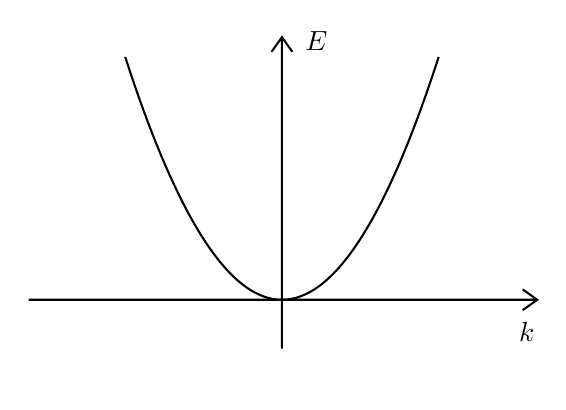
\begin{tikzpicture}[x=0.75pt,y=0.75pt,yscale=-1,xscale=1]
%uncomment if require: \path (0,300); %set diagram left start at 0, and has height of 300

%Shape: Parabola [id:dp9002057271429234] 
\draw   (234.67,67) .. controls (285,223) and (335.33,223) .. (385.67,67) ;
%Shape: Axis 2D [id:dp47011928159342387] 
\draw  (188.17,184) -- (433.17,184)(310.17,57.5) -- (310.17,207.5) (426.17,179) -- (433.17,184) -- (426.17,189) (305.17,64.5) -- (310.17,57.5) -- (315.17,64.5)  ;

% Text Node
\draw (320,53.4) node [anchor=north west][inner sep=0.75pt]    {$E$};
% Text Node
\draw (423,193.4) node [anchor=north west][inner sep=0.75pt]    {$k$};
\end{tikzpicture}
    \caption{自由电子$E-k$曲线}
    \label{fig:free_e_E-k}
\end{figure}

\subsubsection{1. 晶体中薛定谔方程及其解的形式}

单电子近似认为晶体中的电子在与晶格同周期的周期势场中运动。对于一维晶格,$x$处的电势为:
\begin{equation}
    V(x)=V(x+na)\label{eq:cristal_potential}
\end{equation}
其中$n$为整数,$a$为晶格常数。晶体中电子满足薛定谔方程:
\begin{equation}
    -\frac{\hslash^2}{2m_0}\frac{\mathrm{d}^2\psi(x)}{\mathrm{d}x^2}+V(x)\psi(x)=E\psi(x)\label{eq:cristal_schrodinger_eq}
\end{equation}
上式中$V(x)$满足\autoref{eq:cristal_potential}。\autoref{eq:cristal_schrodinger_eq}是晶体电子的基本方程。

可以证明,满足\autoref{eq:cristal_schrodinger_eq}的波函数一定具有如下形式:
\begin{equation}
    \psi_k(x)=u_k(x)\mathrm{e}^{\mathrm{i}kx}\label{eq:bloch_equation}
\end{equation}
式中$k$为波数,$u_k(x)$为与晶格同周期的周期函数:
\begin{equation}
    u_k(x)=u_k(x+na)\quad \text{$n$为整数}
\end{equation}
此结论称为\textbf{布洛赫定理}。具有\autoref{eq:bloch_equation}形式的波函数称为\textbf{布洛赫函数}。

\subsubsection{2. 布里渊区与能带}

晶体中电子处在不同$\bm k$状态,具有不同能量$E(\bm k)$。求解\autoref{eq:cristal_schrodinger_eq}可以得到$E(k)-k$关系曲线。当
\begin{equation}
    k=\frac{n\pi}{a}\quad (n=0,\ \pm 1,\ \pm 2,\cdots)
\end{equation}
时,能量不连续,形成一系列禁带和允带。
\begin{figure}[H]
    \centering
    \includegraphics{energy_band.png}
    \caption{$E(k)-k$关系}
    \label{fig:energy_band}
\end{figure}

\vspace{1ex}可以看到,能量$E(k)$也为$k$的周期函数,周期为$\D\frac{2\pi}{a}$:
\begin{equation}
    E(k)=E\left(k+n\frac{2\pi}{a}\right)
\end{equation}
\vspace{1ex}故$k$和$k+\D n\frac{2\pi}{a}$表示相同的状态,可以只取第一布里渊区$\D -\frac{\pi}{a}<k<\frac{\pi}{a}$中的$k$值描述电子的能量状态,
\vspace{1ex}将其他区域移动$\D n\frac{2\pi}{a}$合并到第一区。这个区域内的$E$是$k$的多值函数,我们称此区域为\textbf{简约布里渊区},区域内波矢为\textbf{简约波矢}。

对于有限晶体需要考虑边界条件。根据周期性边界条件,得到波矢$k$只能取分立值。对边长$L$的立方晶体,波矢$\bm k$的各分量:
\begin{equation}
\begin{split}
    k_x=\frac{2\pi n_x}{L}\quad (n_x=0,\ \pm 1,\ \pm 2,\cdots)\\
    k_y=\frac{2\pi n_y}{L}\quad (n_x=0,\ \pm 1,\ \pm 2,\cdots)\\
    k_z=\frac{2\pi n_z}{L}\quad (n_x=0,\ \pm 1,\ \pm 2,\cdots)
\end{split}
\end{equation}

\subsection{导体,半导体,绝缘体}

固体按其导电性分为导体,半导体,绝缘体。

\section{半导体中电子的运动,有效质量}

\subsection{半导体中的\texorpdfstring{$E(k)$}{E(k)}与\texorpdfstring{$k$}{k}的关系}

半导体中起作用的一般是带底或者带顶的电子,因此只要研究带顶和带底附近的$E(k)-k$关系。

我们用泰勒展开近似地研究能带极值附近$E(k)$与$k$的关系。一维情况下,设能带底位于$k=0$处。

将$E(k)$在$k=0$附近泰勒展开,取到$k^2$项:
\begin{equation}
    E(k)=E(0)+\left(\frac{\mathrm{d}E}{\mathrm{d}k}\right)_{k=0}k+\frac{1}{2}\left(\frac{\mathrm{d^2}E}{\mathrm{d}k^2}\right)_{k=0}k^2+\mathcal{O}(k^3)
\end{equation}
\vspace{1ex}由于在$k=0$时,$\D\left(\frac{\mathrm{d}E}{\mathrm{d}k}\right)_{k=0}\propto (\hslash k)_{k=0}=0$,从而:
\begin{equation}
    E(k)-E(0)=\frac{1}{2}\left(\frac{\mathrm{d}^2E}{\mathrm{d}k^2}\right)_{k=0}k^2\label{eq:E(k)-E(0)}
\end{equation}
其中$E(0)$为带底能量。
令
\begin{equation}
    \frac{1}{m_n^*}=\frac{1}{\hslash^2}\left(\frac{\mathrm{d}^2E}{\mathrm{d}k^2}\right)_{k=0}\label{eq:effect_m}
\end{equation}
将\autoref{eq:effect_m}代入\autoref{eq:E(k)-E(0)},得到带底附近$E(k)$为
\begin{equation}
    E(k)-E(0)=\frac{\hslash^2k^2}{2m_n^*}\label{eq:electron_effect_mass_energy_bottom}
\end{equation}
区别于\autoref{eq:free_e_wave_energy}中的电子惯性质量$m_0$,$m_n^*$称为\textbf{带底电子}的\textbf{有效质量}。由于$E(k)>E(0)$,故$m_n^*$是\textbf{正值}。

同样的,设带顶位于$k=0$处,则在带顶附近得到:
\begin{equation}
    E(k)-E(0)=\frac{1}{2}\left(\frac{\mathrm{d^2}E}{\mathrm{d}k^2}\right)_{k=0}k^2
\end{equation}
令
\begin{equation*}
    \frac{1}{m_n^*}=\frac{1}{\hslash^2}\left(\frac{\mathrm{d}^2E}{\mathrm{d}k^2}\right)_{k=0}
\end{equation*}
则带顶附近$E(k)$为
\begin{equation}
    E(k)-E(0)=\frac{\hslash^2k^2}{2m_n^*}\label{eq:electron_effect_mass_energy_top}
\end{equation}
$m_n^*$称为\textbf{带顶电子}的\textbf{有效质量}。由于$E(k)<E(0)$,$m_n^*$为\textbf{负值}。

\autoref{eq:electron_effect_mass_energy_bottom}和\autoref{eq:electron_effect_mass_energy_top}可见,只要能够确定出有效质量$m_n^*$大小,就能得到能带极值附近的$E(k)-k$关系。

\subsection{半导体中电子的平均速度}

\vspace{1ex}自由电子速度由\autoref{eq:free_e_wave_velocity}确定。由\autoref{eq:free_e_wave_energy}可以求得 $\D\frac{\mathrm{d}E}{\mathrm{d}k}=\frac{\hslash^2k}{m_0}$,
代入
\autoref{eq:free_e_wave_velocity},
\vspace{1ex}得自由电子速度 $\D v=\frac{1}{\hslash}\frac{\mathrm{d}E}{\mathrm{d}k}$。

根据量子力学,电子的运动可以视为波包的运动,波包的群速度即电子的平均速度。设波包由若干角频率$\omega$的波组成,则波包的群速度:
\begin{equation}
    v=\frac{\mathrm{d}\omega}{\mathrm{d}k}\label{eq:wave_group_v}
\end{equation}
又由于角频率$\omega$的波,其粒子能量为$\hslash\omega$,代入\autoref{eq:wave_group_v}:
\begin{equation}
    v=\frac{\mathrm{d}\omega}{\mathrm{d}k}=\frac{1}{\hslash}\frac{\mathrm{d}\hslash\omega}{\mathrm{d}k}=\frac{1}{\hslash}\frac{\mathrm{d}E}{\mathrm{d}k}\label{eq:semi_velocity_energy_relation}
\end{equation}
再代入\autoref{eq:electron_effect_mass_energy_bottom}或\autoref{eq:electron_effect_mass_energy_top},得:
\begin{align}
    v&=\frac{1}{\hslash}\frac{\mathrm{d}}{\mathrm{d}k}\left(E(0)+\frac{\hslash^2k^2}{2m_n^*}\right)\notag\\
    &=\frac{1}{\hslash}\frac{\hslash^2k}{m_n^*}\notag\\
    &=\frac{\hslash k}{m_n^*}\label{eq:semi_velocity_k_m_eff_relation}
\end{align}
带底$m_n^*>0$,$k$为正值时,$v$为正值;带顶$m_n^*《0$,$k$为正值时,$v$为负值

\subsection{半导体中电子的加速度}

在强度$\mathscr{E}$的外电场下,电子受到$f=-q\mathscr{E}$的电场力,$\mathrm{d}t$时间内产生位移$\mathrm{d}s$。外力做功产生的能量变化:
\begin{equation}
    \mathrm{d}E=f\mathrm{d}s=fv\mathrm{d}t
\end{equation}
代入\autoref{eq:semi_velocity_energy_relation},得:
\begin{align}
    &\mathrm{d}E=\frac{f}{\hslash}\frac{\mathrm{d}E}{\mathrm{d}k}\mathrm{d}t\\
    \Longrightarrow&f=\hslash\frac{\mathrm{d}k}{\mathrm{d}t}\label{eq:force_k_t_relation}
\end{align}
上式说明了外力$f$作用下,波矢$k$会发生改变。

电子加速度:
\begin{equation}
    a=\frac{\mathrm{d}v}{\mathrm{d}t}=\frac{1}{\hslash}\frac{\mathrm{d}}{\mathrm{d}t}\frac{\mathrm{d}E}{\mathrm{d}k}=\frac{1}{\hslash}\frac{\mathrm{d}k}{\mathrm{d}t}\frac{\mathrm{d}^2E}{\mathrm{d}k^2}=\frac{f}{\hslash^2}\frac{\mathrm{d}^2E}{\mathrm{d}k^2}
\end{equation}
由
\begin{equation}
    \frac{1}{m_n^*}=\frac{1}{\hslash^2}\frac{\mathrm{d}^2E}{\mathrm{d}k^2}\quad \text{or}\quad m_n^*=\frac{\hslash^2}{\D\frac{\mathrm{d}^2E}{\mathrm{d}k^2}}
\end{equation}
\vspace{1ex}得:
\begin{equation}
    a=\frac{f}{m_n^*}=-\frac{q\mathscr{E}}{m_n^*}
    \label{eq:accel_force}
\end{equation}
可以看出,引入电子有效质量后,半导体电子的运动与牛顿第二定律类似。

\section{本征半导体中的空穴}

在$K=0$下,纯净半导体的价带被价电子填满,导带为空。一定温度下,价带顶部电子被激发到导带。被激发的电子参与导电。价带由于缺少电子,形成带正电的准粒子,即\textbf{空穴}。

空穴具有一个单位的正电荷$+q$,有效质量$m_p^*$有:
\begin{equation}
    m_p^*=-m_n^*
\end{equation}
在外电场$\mathscr{E}$下,空穴的加速度
\begin{equation}
    a=\frac{q\mathscr{E}}{m_p^*}=\frac{f}{m_p^*}
\end{equation}

\chapter{回旋共振与导带和价带结构}

\section{回旋共振}

\subsection{\texorpdfstring{$k$}{k}空间等能面}

根据1.3节,$k=0$在导带底电子,有:
\begin{equation}
    E(k)-E(0)=\frac{\hslash^2k^2}{2m_n^*}
\end{equation}
对于价带顶的空穴,同样有:
\begin{equation}
    E(k)-E(0)=-\frac{\hslash^2k^2}{2m_p^*}
\end{equation}

对于三维晶体,$\bm k$有$k_x,\ k_y,\ k_z$三个分量,满足:
\begin{equation}
    k^2=k_x^2+k_y^2+k_z^2
\end{equation}
代入导带底位于$\bm k=\bm 0$,能量为$E(0)$的情况,有:
\begin{equation}
    E(\bm k)-E(0)=\frac{\hslash^2}{2m_n^*}\left(k_x^2+k_y^2+k_z^2\right)
\end{equation}

对于各向异性的晶体,$E(\bm k)$和$\bm k$的关系在$\bm k$沿不同方向上并不完全一致。

根据
\begin{equation}
    \frac{1}{m_n^*}=\frac{1}{\hslash^2}\frac{\mathrm{d}^2E}{\mathrm{d}\bm k^2}
\end{equation}
\vspace{1ex}可知,$\D\frac{1}{m_n^*}$是一个二阶张量:
\begin{equation}
    \left(\frac{1}{m_n^*}\right)_{ij}=
    \frac{1}{\hslash^2}\frac{\partial^2E}{\partial k_i\partial k_j}
    ,\quad \left(i,\ j\ \text{取遍}\ 1,\ 2,\ 3\right)
\end{equation}

\vspace{1ex}我们对$\D\left(\frac{1}{m_n^*}\right)_{ij}$作正交变换,取$\D\left(\frac{1}{m_n^*}\right)_{ij}$仅有对角元素时的基矢为$\bm k_x,\ \bm k_y,\ \bm k_z$。此时记$m_x^*,\ m_y^*,\ m_z^*$分别为$\bm k_x,\ \bm k_y,\ \bm k_z$方向上的电子有效质量:
\begin{equation}
    \left\{
    \begin{aligned}
        \frac{1}{m_x^*}=\frac{1}{\hslash^2}\left(\frac{\partial^2E}{\partial k_x^2}\right)_{k_0}\\
        \frac{1}{m_y^*}=\frac{1}{\hslash^2}\left(\frac{\partial^2E}{\partial k_y^2}\right)_{k_0}\\
        \frac{1}{m_z^*}=\frac{1}{\hslash^2}\left(\frac{\partial^2E}{\partial k_z^2}\right)_{k_0}
        \end{aligned}
    \right.
\end{equation}

设导带底位于$\bm k_0$,能量为$E(k_0)$。在$k_0$附近将$E(k_0)$泰勒展开,取到二次项:
\begin{equation}
    E(k)=E(k_0)+\frac{\hslash^2}{2}\left(\frac{(k_x-k_{0x})^2}{m_x^*}+\frac{(k_y-k_{0y})^2}{m_y^*}+\frac{(k_z-k_{0z})^2}{m_z^*}\right)
    \label{eq:homo_energy_equation}
\end{equation}
即: 
\begin{equation}
    \frac{\quad(k_x-k_{0x})^2\quad}{\D \frac{2m_x^*\left(E-E_c\right)}{\hslash^2}}+
    \frac{\quad(k_y-k_{0y})^2\quad}{\D \frac{2m_y^*\left(E-E_c\right)}{\hslash^2}}+
    \frac{\quad(k_z-k_{0z})^2\quad}{\D \frac{2m_z^*\left(E-E_c\right)}{\hslash^2}}=1
    \label{eq:homo_energy_eclipse_equation}
\end{equation}
\autoref{eq:homo_energy_eclipse_equation}是个椭圆方程,即等能面是围绕$\bm k_0$的一系列椭球面。

\subsection{回旋共振}

半导体置于磁感应强度$\bm B$的磁场中,电子初速度为$\bm v$,磁场力$\bm f$:
\begin{equation}
    \bm f=-q\bm v\times\bm B
\end{equation}
$\bm v$和$\bm B$夹角为$\theta$:
\begin{equation}
    \theta=\arccos{\left(\frac{\bm v\cdot\bm B}{\left|v\right|\left|B\right|}\right)}
\end{equation}
则$f$的大小为:
\begin{equation}
    f=qvB\sin{\theta}=qv_{\perp}B,\quad v_{\perp}=v\sin{\theta}
\end{equation}
电子的轨迹在沿磁场方向为速度$v_{\parallel}=v\cos{\theta}$的匀速运动,在垂直于磁场的平面内作匀速圆周运动,总体的运动轨迹为以螺旋线进动。

设圆周半径$r$,回旋频率为$\omega_c$,则有
\begin{equation}
    v_{\perp}=r\omega_c
\end{equation}
向心加速度$a$:
\begin{equation}
    a=\frac{v_{\perp}^2}{r}
\end{equation}
代入\autoref{eq:accel_force},得
\begin{align}
    &\frac{v_{\perp}^2}{r}=\frac{f}{m_n^{*}}=\frac{qv_{\perp}B}{m_n^*}\notag\\
    \Longrightarrow&v_{\perp}=r\omega_c=\frac{qBr}{m_n^*}\notag\\
    \Longrightarrow&\omega_c=\frac{qB}{m_n^*}\label{eq:ball-cyclotron-resonance}
\end{align}
将电磁波通过半导体样品,当交变电磁场的角频率$\omega$等于回旋频率$\omega_c$时,就会发生共振吸收。测出共振吸收时的电磁波角频率$\omega$和磁感应强度$B$,便可以算出有效质量$m_n$。

若等能面是椭球面,则有效质量也是各向异性的。设沿$k_x,\ k_y,\ k_z$轴方向分别是$m_x^*,\ m_y^*,\ m_z^*$。设$\bm B$沿$k_x,\ k_y,\ k_z$轴的方向余弦为$\alpha,\ \beta,\ \gamma$,则电子受力:
\begin{equation}
\left\{
    \begin{aligned}
        f_x=-qB\left(v_y\gamma-v_z\beta\right)\\
        f_y=-qB\left(v_z\alpha-v_x\gamma\right)\\
        f_z=-qB\left(v_x\beta-v_y\alpha\right)
    \end{aligned}
\right.
\end{equation}
得到运动方程:
\begin{equation}
    \left\{
    \begin{aligned}
        m_x^*\frac{\mathrm{d}v_x}{\mathrm{d}t}+qB\left(v_y\gamma-v_z\beta\right)=0\\
        m_y^*\frac{\mathrm{d}v_y}{\mathrm{d}t}+qB\left(v_z\alpha-v_x\gamma\right)=0\\
        m_z^*\frac{\mathrm{d}v_z}{\mathrm{d}t}+qB\left(v_x\beta-v_y\alpha\right)=0
    \end{aligned}
    \right.
\end{equation}
电子作周期运动,取解:
\begin{equation}
    \left\{
    \begin{aligned}
        v_x=v_x'\mathrm{e}^{\mathrm{i}\omega_ct}\\
        v_y=v_y'\mathrm{e}^{\mathrm{i}\omega_ct}\\
        v_z=v_z'\mathrm{e}^{\mathrm{i}\omega_ct}
    \end{aligned}
    \right.
\end{equation}
代入,得:
\begin{equation}
    \left\{
    \begin{aligned}
        \mathrm{i}\omega_cv_x'+\frac{qB}{m_x^*}\gamma v_y'-\frac{qB}{m_x^*}\beta v_z'=0\\
        -\frac{qB}{m_y^*}\gamma v_x'+\mathrm{i}\omega_cv_y'+\frac{qB}{m_y^*}\alpha v_z'=0\\
        \frac{qB}{m_z^*}\beta v_x'-\frac{qB}{m_z^*}\alpha v_y'+\mathrm{i}\omega_cv_z'=0
    \end{aligned}
    \right.
\end{equation}
要使$v_x',\ v_y',\ v_z'$有不全为零的解,其系数行列式为零:
\begin{equation}
    \begin{vmatrix}
        \mathrm{i}\omega_c & \D\frac{qB}{m_x^*}\gamma & \D-\frac{qB}{m_x^*}\beta\vspace{1ex}\\
        \D-\frac{qB}{m_y^*}\gamma & \mathrm{i}\omega_c & \D\frac{qB}{m_y^*}\alpha\vspace{1ex}\\
        \D\frac{qB}{m_z^*}\beta & \D-\frac{qB}{m_z^*}\alpha & \mathrm{i}\omega_c
    \end{vmatrix}
    =0
\end{equation}
解得电子回旋频率$\omega_c$:
\begin{equation}
    \omega_c=\frac{qB}{m_n^*}
\end{equation}
其中
\begin{equation}
    \frac{1}{m_n^*}=\sqrt{\frac{m_x^*\alpha^2+m_y^*\beta^2+m_z^*\gamma^2}{m_x^*m_y^*m_z^*}}\label{eq:ecllipse-cyclotron-resonance-eff-mass}
\end{equation}
交变电磁场的角频率$\omega$等于$\omega_c$时,发生共振吸收。

\section{硅和锗的能带结构}

\subsection{硅和锗的导带结构}

对于等能面为球面的晶体,由\autoref{eq:ball-cyclotron-resonance},改变磁场方向仅有一个吸收峰。硅的回旋共振实验中:
\begin{enumerate}[(1)]
    \item $\bm B$沿$[1\ 1\ 1]$方向,有一个吸收峰;
    \item $\bm B$沿$[1\ 1\ 0]$方向,有两个吸收峰;
    \item $\bm B$沿$[1\ 0\ 0]$方向,有两个吸收峰;
    \item $\bm B$沿任意取向,有三个吸收峰。
\end{enumerate}
显然不是各向同性的。我们认为硅导带底附近等能面是沿$[1\ 0\ 0]$方向的旋转椭球面,且椭圆长轴沿此方向,则与实验事实吻合。此时的导带最小值不在$\bm k$空间原点,而在$[1\ 0\ 0]$方向上,根据对称性,也出现在$[\Bar{1}\ 0\ 0],\ [0\ 1\ 0],\ [0\ \Bar{1},\ 0],\ [0\ 0\ 1],\ [0\ 0\ \Bar{1}]$方向上,如\autoref{fig:homo-energy-phase}。
\begin{figure}[H]
    \centering
\tikzset{every picture/.style={line width=0.75pt}} %set default line width to 0.75pt        

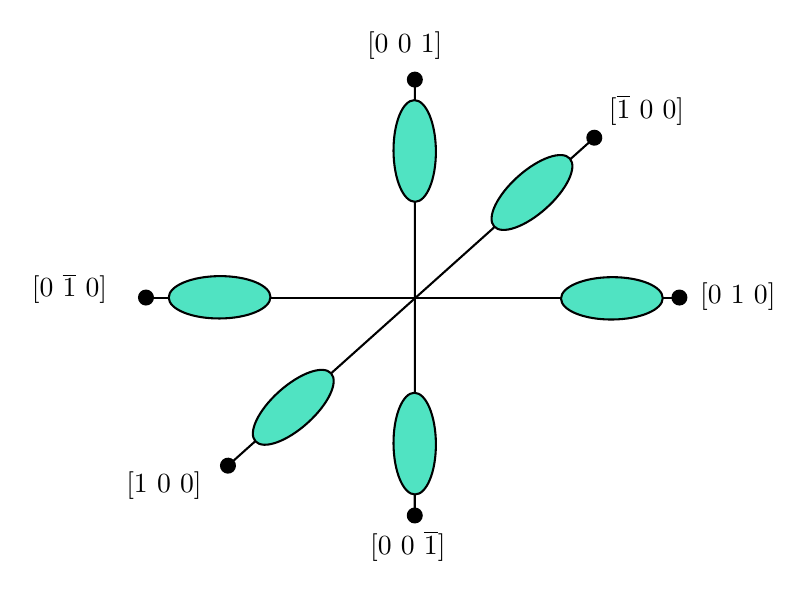
\begin{tikzpicture}[x=0.75pt,y=0.75pt,yscale=-1,xscale=1]
%uncomment if require: \path (0,300); %set diagram left start at 0, and has height of 300

%Straight Lines [id:da22604722746412387] 
\draw    (264.67,259.75) -- (264.7,49.75) ;
\draw [shift={(264.7,49.75)}, rotate = 270.01] [color={rgb, 255:red, 0; green, 0; blue, 0 }  ][fill={rgb, 255:red, 0; green, 0; blue, 0 }  ][line width=0.75]      (0, 0) circle [x radius= 3.35, y radius= 3.35]   ;
\draw [shift={(264.67,259.75)}, rotate = 270.01] [color={rgb, 255:red, 0; green, 0; blue, 0 }  ][fill={rgb, 255:red, 0; green, 0; blue, 0 }  ][line width=0.75]      (0, 0) circle [x radius= 3.35, y radius= 3.35]   ;
%Straight Lines [id:da7464742627624705] 
\draw    (135.17,154.75) -- (392.17,154.75) ;
\draw [shift={(392.17,154.75)}, rotate = 0] [color={rgb, 255:red, 0; green, 0; blue, 0 }  ][fill={rgb, 255:red, 0; green, 0; blue, 0 }  ][line width=0.75]      (0, 0) circle [x radius= 3.35, y radius= 3.35]   ;
\draw [shift={(135.17,154.75)}, rotate = 0] [color={rgb, 255:red, 0; green, 0; blue, 0 }  ][fill={rgb, 255:red, 0; green, 0; blue, 0 }  ][line width=0.75]      (0, 0) circle [x radius= 3.35, y radius= 3.35]   ;
%Straight Lines [id:da8922617180358392] 
\draw    (174.67,235.75) -- (351.17,77.75) ;
\draw [shift={(351.17,77.75)}, rotate = 318.17] [color={rgb, 255:red, 0; green, 0; blue, 0 }  ][fill={rgb, 255:red, 0; green, 0; blue, 0 }  ][line width=0.75]      (0, 0) circle [x radius= 3.35, y radius= 3.35]   ;
\draw [shift={(174.67,235.75)}, rotate = 318.17] [color={rgb, 255:red, 0; green, 0; blue, 0 }  ][fill={rgb, 255:red, 0; green, 0; blue, 0 }  ][line width=0.75]      (0, 0) circle [x radius= 3.35, y radius= 3.35]   ;
%Shape: Ellipse [id:dp14232987209042292] 
\draw  [fill={rgb, 255:red, 80; green, 227; blue, 194 }  ,fill opacity=1 ] (187.9,224) .. controls (184.14,219.8) and (189.25,209.07) .. (199.32,200.04) .. controls (209.39,191) and (220.61,187.08) .. (224.37,191.27) .. controls (228.14,195.47) and (223.03,206.2) .. (212.95,215.23) .. controls (202.88,224.27) and (191.67,228.19) .. (187.9,224) -- cycle ;
%Shape: Ellipse [id:dp5560073327977961] 
\draw  [fill={rgb, 255:red, 80; green, 227; blue, 194 }  ,fill opacity=1 ] (302.9,120.5) .. controls (299.14,116.3) and (304.25,105.57) .. (314.32,96.54) .. controls (324.39,87.5) and (335.61,83.58) .. (339.37,87.77) .. controls (343.14,91.97) and (338.03,102.7) .. (327.95,111.73) .. controls (317.88,120.77) and (306.67,124.69) .. (302.9,120.5) -- cycle ;
%Shape: Ellipse [id:dp7111731340388567] 
\draw  [fill={rgb, 255:red, 80; green, 227; blue, 194 }  ,fill opacity=1 ] (335.14,155.27) .. controls (335.11,149.63) and (346.05,145) .. (359.58,144.93) .. controls (373.11,144.85) and (384.11,149.36) .. (384.14,155) .. controls (384.17,160.64) and (373.22,165.27) .. (359.69,165.34) .. controls (346.16,165.42) and (335.17,160.91) .. (335.14,155.27) -- cycle ;
%Shape: Ellipse [id:dp8131792583845494] 
\draw  [fill={rgb, 255:red, 80; green, 227; blue, 194 }  ,fill opacity=1 ] (146.14,154.77) .. controls (146.11,149.13) and (157.05,144.5) .. (170.58,144.43) .. controls (184.11,144.35) and (195.11,148.86) .. (195.14,154.5) .. controls (195.17,160.14) and (184.22,164.77) .. (170.69,164.84) .. controls (157.16,164.92) and (146.17,160.41) .. (146.14,154.77) -- cycle ;
%Shape: Ellipse [id:dp3883439769649071] 
\draw  [fill={rgb, 255:red, 80; green, 227; blue, 194 }  ,fill opacity=1 ] (264.45,59.64) .. controls (270.09,59.59) and (274.74,70.53) .. (274.85,84.06) .. controls (274.95,97.59) and (270.46,108.59) .. (264.82,108.63) .. controls (259.18,108.68) and (254.53,97.74) .. (254.43,84.21) .. controls (254.33,70.68) and (258.82,59.68) .. (264.45,59.64) -- cycle ;
%Shape: Ellipse [id:dp974977775233371] 
\draw  [fill={rgb, 255:red, 80; green, 227; blue, 194 }  ,fill opacity=1 ] (264.45,200.64) .. controls (270.09,200.59) and (274.74,211.53) .. (274.85,225.06) .. controls (274.95,238.59) and (270.46,249.59) .. (264.82,249.63) .. controls (259.18,249.68) and (254.53,238.74) .. (254.43,225.21) .. controls (254.33,211.68) and (258.82,200.68) .. (264.45,200.64) -- cycle ;

% Text Node
\draw (240.17,25.23) node [anchor=north west][inner sep=0.75pt]    {$[ 0\ 0\ 1]$};
% Text Node
\draw (241.67,265.73) node [anchor=north west][inner sep=0.75pt]    {$[ 0\ 0\ \overline{1}]$};
% Text Node
\draw (400.67,146.23) node [anchor=north west][inner sep=0.75pt]    {$[ 0\ 1\ 0]$};
% Text Node
\draw (78.67,141.73) node [anchor=north west][inner sep=0.75pt]    {$[ 0\ \overline{1} \ 0]$};
% Text Node
\draw (356.67,55.73) node [anchor=north west][inner sep=0.75pt]    {$[ \overline{1}\ 0\ 0]$};
% Text Node
\draw (124.17,237.23) node [anchor=north west][inner sep=0.75pt]    {$[1 \ 0\ 0]$};
\end{tikzpicture}
    \caption{硅导带等能面}
    \label{fig:homo-energy-phase}
\end{figure}

由\autoref{eq:homo_energy_equation},极值附近能量$E^s(\bm k)$为:
\begin{equation}
    E^s(\bm k)=E_c+\frac{\hslash^2}{2}\left(\frac{(k_x-k_{0x}^s)^2}{m_x^*}+\frac{(k_y-k_{0y}^s)^2}{m_y^*}+\frac{(k_z-k_{0z}^s)^2}{m_z^*}\right)
\end{equation}

取$E_c$为能量零点,$\bm k_0^s$为坐标原点,取$k_1,\ k_2,\ k_3$三个直角坐标轴分别沿椭球主轴方向,其中$k_3$沿长轴方向$(<100>)$,等能面为绕$k_3$的旋转椭球面。此时沿$k_1,\ k_2$轴的有效质量相同,如\autoref{fig:k-space-B}。

令$m_x^*=m_y^*=m_t$为\textbf{横向有效质量},$m_z^*=m_l$为\textbf{纵向有效质量}。等能面方程化为:
\begin{equation}
    E(\bm k)=\frac{\hslash^2}{2}\left[\frac{k_1^2+k_2^2}{m_t}+\frac{k_3^2}{m_l}\right]
\end{equation}
\begin{figure}[ht]
    \centering
\tikzset{every picture/.style={line width=0.75pt}} %set default line width to 0.75pt        

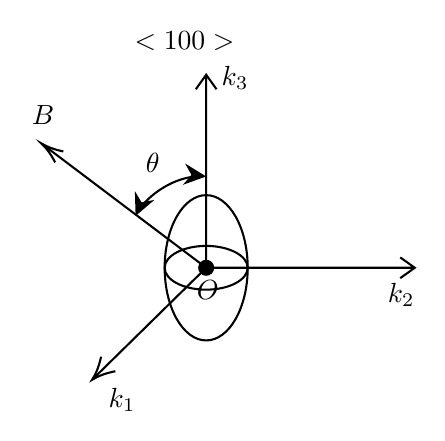
\begin{tikzpicture}[x=0.75pt,y=0.75pt,yscale=-1,xscale=1]
%uncomment if require: \path (0,300); %set diagram left start at 0, and has height of 300

%Shape: Axis 2D [id:dp8786621681916096] 
\draw  (260.67,136.08) -- (361.17,136.08)(260.67,43.08) -- (260.67,136.08) -- cycle (354.17,131.08) -- (361.17,136.08) -- (354.17,141.08) (255.67,50.08) -- (260.67,43.08) -- (265.67,50.08)  ;
%Straight Lines [id:da8481261784727727] 
\draw    (260.67,136.08) -- (207.09,188.68) ;
\draw [shift={(205.67,190.08)}, rotate = 315.53] [color={rgb, 255:red, 0; green, 0; blue, 0 }  ][line width=0.75]    (10.93,-4.9) .. controls (6.95,-2.3) and (3.31,-0.67) .. (0,0) .. controls (3.31,0.67) and (6.95,2.3) .. (10.93,4.9)   ;
\draw [shift={(260.67,136.08)}, rotate = 135.53] [color={rgb, 255:red, 0; green, 0; blue, 0 }  ][fill={rgb, 255:red, 0; green, 0; blue, 0 }  ][line width=0.75]      (0, 0) circle [x radius= 3.35, y radius= 3.35]   ;
%Shape: Ellipse [id:dp9193111334407007] 
\draw   (260.67,101.08) .. controls (271.71,101.08) and (280.67,116.75) .. (280.67,136.08) .. controls (280.67,155.41) and (271.71,171.08) .. (260.67,171.08) .. controls (249.62,171.08) and (240.67,155.41) .. (240.67,136.08) .. controls (240.67,116.75) and (249.62,101.08) .. (260.67,101.08) -- cycle ;
%Shape: Ellipse [id:dp9104121259221969] 
\draw   (240.67,136.08) .. controls (240.67,130.26) and (249.62,125.54) .. (260.67,125.54) .. controls (271.71,125.54) and (280.67,130.26) .. (280.67,136.08) .. controls (280.67,141.91) and (271.71,146.62) .. (260.67,146.62) .. controls (249.62,146.62) and (240.67,141.91) .. (240.67,136.08) -- cycle ;
%Straight Lines [id:da5005870637429592] 
\draw    (260.67,136.08) -- (182.76,77.29) ;
\draw [shift={(181.17,76.08)}, rotate = 37.04] [color={rgb, 255:red, 0; green, 0; blue, 0 }  ][line width=0.75]    (10.93,-3.29) .. controls (6.95,-1.4) and (3.31,-0.3) .. (0,0) .. controls (3.31,0.3) and (6.95,1.4) .. (10.93,3.29)   ;
%Curve Lines [id:da2319691018502339] 
\draw    (228.2,108.32) .. controls (233.34,100.54) and (245.58,92.11) .. (257.72,91.95) ;
\draw [shift={(260.67,92.08)}, rotate = 185.91] [fill={rgb, 255:red, 0; green, 0; blue, 0 }  ][line width=0.08]  [draw opacity=0] (10.72,-5.15) -- (0,0) -- (10.72,5.15) -- (7.12,0) -- cycle    ;
\draw [shift={(226.67,111.08)}, rotate = 293.96] [fill={rgb, 255:red, 0; green, 0; blue, 0 }  ][line width=0.08]  [draw opacity=0] (10.72,-5.15) -- (0,0) -- (10.72,5.15) -- (7.12,0) -- cycle    ;

% Text Node
\draw (212.17,192.4) node [anchor=north west][inner sep=0.75pt]    {$k_{1}$};
% Text Node
\draw (346.67,141.9) node [anchor=north west][inner sep=0.75pt]    {$k_{2}$};
% Text Node
\draw (266.67,37.4) node [anchor=north west][inner sep=0.75pt]    {$k_{3}$};
% Text Node
\draw (224.67,20.9) node [anchor=north west][inner sep=0.75pt]    {$< 100 >$};
% Text Node
\draw (175.17,56.4) node [anchor=north west][inner sep=0.75pt]    {$\bm B $};
% Text Node
\draw (230.17,79.4) node [anchor=north west][inner sep=0.75pt]    {$\theta $};
% Text Node
\draw (254.67,140.9) node [anchor=north west][inner sep=0.75pt]    {$O$};
\end{tikzpicture}
    \caption{$\bm k$空间取向}
    \label{fig:k-space-B}
\end{figure}

我们选取$k_1$使得$\bm B$位于$k_1$和$k_3$组成的平面内,并与$k_3$成$\theta$角。此时$\bm B$的方向余弦:
\begin{equation}
    \alpha=\sin\theta,\ \beta=0,\ \gamma=\cos\theta
\end{equation}
代入\autoref{eq:ecllipse-cyclotron-resonance-eff-mass},得:
\begin{equation}
    m_n^*=m_t\sqrt{\frac{m_l}{m_t\sin^2\theta+m_l\cos^2\theta}}\label{eq:silicon-cyclotron-resonance-eff-mass}
\end{equation}

\begin{enumerate}[(1)]
    \item \vspace{1ex}当$\bm B$沿$[1\ 1\ 1]$方向,则与$6$个$<100>$方向夹角均为$\cos^2\theta=\D\frac{1}{3}$,因此$\sin^2\theta=\D\frac{2}{3}$,代入\autoref{eq:silicon-cyclotron-resonance-eff-mass},得:
    \begin{equation}
        m_n^*=m_t\sqrt{\frac{3m_l}{2m_t+m_l}}
    \end{equation}
    \vspace{1ex}由$\omega=\omega_c=\D\frac{qB}{m_n^*}$可知,$m_n^*$只有一个值,只能观察到一个吸收峰。
    \item $\bm B$沿$[1\ 1\ 0]$方向,此时$\bm B$与$[1\ 0\ 0],\ [\overline{1}\ 0\ 0],\ [0\ 1\ 0],\ [0,\ \overline{1},\ 0]$夹角$\cos^2\theta_1=\D\frac{1}{2},\ \sin^2\theta_1=\D\frac{1}{2}$,与$[0\ 0\ 1],\ [0\ 0\ \overline{1}]$夹角有$\cos^2\theta_2=0,\ \sin^2\theta_2=1$,代入\autoref{eq:silicon-cyclotron-resonance-eff-mass},相应的有效质量分别为:
    \begin{align}
        m_{n1}^*&=m_t\sqrt{\frac{2m_l}{m_t+m_l}}\\
        m_{n2}^*&=\sqrt{m_lm_t}
    \end{align}
    存在$2$个不同的$m_n^*$值,故有两个吸收峰。
    \item $\bm B$沿$[1\ 0\ 0]$方向,此时$\bm B$与$[1\ 0\ 0],\ [\overline{1}\ 0\ 0]$夹角给出$\cos^2\theta_1=1,\ \sin^2\theta_=0$,
    与
    $[0\ 1\ 0]$
    ,\ $[0,\ \overline{1},\ 0]$
    ,\ $[0\ 0\ 1]$
    ,\ $[0\ 0\ \overline{1}]$
    夹角有$\cos^2\theta_2=0,\ \sin^2\theta_2=1$。代入\autoref{eq:silicon-cyclotron-resonance-eff-mass},相应的有效质量分别为:
    \begin{align}
        m_n^*&=m_t\\
        m_n^*&=\sqrt{m_lm_t}
    \end{align}
    存在$2$个不同的$m_n^*$值,故也有两个吸收峰。
    \item $\bm B$沿任意方向时,与$<100>$夹角给出三种$\cos^2\theta$值,因此有三种不同的$m_n^*$,可以观察到三个吸收峰。
\end{enumerate}
上述讨论与实验结果相符,因此硅导带底附近等能面是沿$[1\ 0\ 0]$方向的旋转椭球面。

对于n型锗的实验结果显示,锗的导带极值位于$<111>$方向。






















